\documentclass{article}
\usepackage{amsmath, amsthm, amssymb} % maths stuffs
\usepackage[english, main=greek]{babel} 
\usepackage[a4paper, total={6in, 10in}]{geometry}
\usepackage{graphicx}  % for images
\usepackage{subcaption} % for multiple images in the same figure
\usepackage{titling}
\usepackage[unicode]{hyperref} % enable hyperlink
\usepackage{xcolor}

% 5.1 αντιστοιψισε πηνια τασης \ εντασης με Π1 Π2
\hypersetup{
    colorlinks,
    linkcolor={red!50!black},
    citecolor={blue!50!black},
    urlcolor={blue!80!black}
}


\setlength{\parindent}{0pt}
\setlength{\parskip}{5pt}

\title{72 (περίπου) Ερωτήσεις Συστήματα Μετρήσεων}
\author{\foreignlanguage{english}{PacoPacorius}}
\date{Απρίλιος 2021}

\begin{document}
\maketitle

\renewcommand{\abstractname}{Εισαγωγικό σημείωμα}
\begin{abstract}
    Συνάδελφε! Αυτό το \foreignlanguage{english}{pdf} είναι βασισμένο στη δουλεία του \foreignlanguage{english}{RioCompiler}, και το 
    \foreignlanguage{english}{pdf} με τις 72 ερωτήσεις που είχε κάνει. Ουσιαστικά απλά πήρα τις ίδιες ερωτήσεις, τις έβαλα στη σειρά και τις ταξινόμησα με βάση τα 
    κεφάλαια στο βιβλίο του Πετρίδη, ξαναέγραψα (σχεδόν) όλες τις απαντήσεις από την αρχή κάνοντας τις πιο λιτές και άμεσες, πρόσθεσα πληροφορίες όπου το θεώρησα αναγκαίο. 
    Έβαλα έξτρα σχήματα, τα σχήματα που είχε το \foreignlanguage{english}{pdf} του \foreignlanguage{english}{RioCompiler} τα έβαλα αλλά πιο καθαρά, έβαλα παραπομπές 
    σε σελίδες στο βιβλίο του Πετρίδη για κάθε ερώτηση (για ασκήσεις έχω και από πού είναι η άσκηση και πού να βρεις τους τύπους) αν θες να διαβάσεις κάτι με περισσότερη 
    λεπτομέρεια για κατανόηση και γενικά το έχω καθαρογράψει και σουλουπώσει αρκετά μπορώ να πω. 
\newline
    Συνειδητοποίησα μόλις το τελείωσα ότι η δουλειά του \foreignlanguage{english}{RioCompiler} ήταν συγκέντρωση δύο μαθημάτων ΠΠΣ, οπότε δεν ξέρω κατά πόσο αυτά που 
    βρίσκονται εδώ είναι εντός της ύλης ΝΠΣ, αλλά από,τι καταλαβαίνω πρέπει το $90\%$ να είναι ακόμα εντός ύλης, εξάλλου ξέρω παιδιά που από αυτό διαβάσανε για να δώσουν
    Συστήματα Μετρήσεων και δεν είχαν κάποιο ιδιαίτερο πρόβλημα σχετικά. Απλά τους βγήκε λίγο η πίστη γιατί εκείνο το \foreignlanguage{english}{pdf} είναι λίγο χαώδες και
    ό,τι να ναι.
\newline
    Για \foreignlanguage{english}{updates} $/$ \foreignlanguage{english}{feedback} και λοιπά πάνε στο \foreignlanguage{english}{\href{https://github.com/PacoPacorius/sis-metrisewn-72-erwtiseis-remaster}{GitHub repository}} 
    αυτόυ του \foreignlanguage{english}{pdf}. Εκεί μπορείς να βρεις και αυτό το \foreignlanguage{english}{pdf} το \foreignlanguage{english}{source code} του αρχείου σε
    \foreignlanguage{english}{LaTeX} και όλα τα σχήματα που χρησιμοποιώ σε περίπτωση που θες να το πειράξεις, να το κάνεις \foreignlanguage{english}{compile} μόνος σου
    κλπ κλπ.
\newline
    Αυτά από μένα, καλό κουράγιο συνάδελφε!
\end{abstract}

%\chapter{Μέρος Α}
\section{Σφάλματα Μετρήσεων}

\subsection{Ποιά είναι το κυριότερα είδη σφαλμάτων?}
Τα σφάλματα χωρίζονται σε συστηματικά και τυχαία. Τα συστηματικά οφείλονται στην επίδραση του περιβάλλοντος, στις διάφορες ατέλειες
του οργάνου και στις αδυναμίες των μεθόδων μέτρησης. Χωρίζονται σε στατικά (σφάλμα σε μέτρηση όταν το όργανο είναι σε ισορροπία) και δυναμικά (σφάλμα σε μέτρηση όταν το
μετρούμενο μέγεθος μεταβάλλεται γρήγορα σε σχέση με το μεταβατικό φαινόμενο του οργάνου).

\emph{Σελ. 22, 24}

\subsection{Σε τι διαφέρει η ακρίβεια από την ακρίβεια διασποράς?}
Η ακρίβεια περιγράφει κατά πόσο η ένδειξη ενός οργάνου προσεγγίζει την πραγματική τιμή του μετρούμενου μεγέθους. Ακρίβεια διασποράς λέγεται η διασπορά ενδείξεων ενός 
οργάνου σε επαναλαμβανόμενες μετρήσεις.

\emph{Σελ. 24}

\subsection{Τι είναι η ευαισθησία ενός οργάνου?}
Ευαισθησία είναι ο λόγος της μεταβολής της απόκρισης προς τη μεταβολή της διέγερσης.

\emph{Σελ. 25}

\subsection{Τι σημαίνει διακριτική ικανότητα οργάνου?}
Διακριτική ικανότητα οργάνου λέγεται η μικρότερη δυνατή μεταβολή της μετρούμενης ποσότητας που μπορεί να γίνει αντιληπτή από το όργανο.

\emph{Σελ. 25}
\subsection{Τι είναι η πόλωση οργάνου?}
Πόλωση οργάνου ονομάζεται η τάση του οργάνου να δίνει διαφορετική ένδειξη από την πραγματική τιμή κατά μια σταθερή ποσότητα. Μπορεί να είνα θετική ή αρνητική.

\emph{Σελ. 25}

\subsection{Πώς ορίζεται η κλάση ενός οργάνου?}
Είναι η ποσότητα $G=100*\frac{\Delta x_m}{x_T}$, όπου $\Delta x_m$ μέγιστο απόλυτο σφάλμα, $x_T$ μέγιστη ένδειξη οργάνου. 

\emph{Σελ. 26}

\subsection{Γιατί πρέπει οι ενδείξεις των οργάνων να είναι όσο το δυνατό στο τελευταίο τρίτο της κλίμακας?}
Γιατί το μέγιστο σχετικό σφάλμα της ένδειξης είναι μεγάλο όταν οι ενδείξεις είναι στην αρχή της κλίμακας.

\emph{Σελ. 27}

\subsection{\emph{(Σεπ. 2013)} Ένας ηλεκτροκινητήρας για ορισμένες συνθήκες λειτουργίας απορροφά ηλεκτρική ισχύ $1KW$ και παράγει μηχανική ισχύ $0,9HP$. Αν η μηχανική 
ισχύ μετρήθηκε με μέγιστο σχετικό σφάλμα $2\%$ και η ηλεκτρική ισχύς με βαττόμετρο κλάσης $1\%$ και μέγιστης κλίμακας $1,5KW$ να υπολογιστεί το μέγιστο απόλυτο και 
σχετικό σφάλμα του βαθμού απόδοσης του κινητήρα.}

\begin{align*}
    & x_1 = P_{in} = 1KW\; \text{Ηλεκτρική ισχύς} \\
    & x_2 = P_{out} = 0.9HP = 0.9*745.7 = 671.13W\; \text{Μηχανική ισχύς} \\
    \intertext{Μέτρηση ηλεκτρικής ισχύος:}
    & G = 100*|E_{\text{ενδ}1}| \Rightarrow 1 = 100*|E_{\text{ενδ}1}| \Rightarrow E_{\text{ενδ}1} = 0.01 \\
    & E_{\text{ενδ}1} = \frac{\Delta x_{1m}}{x_1} \Rightarrow \Delta x_{1m} = 0.01 * 1.5KW = 0.015KW \\ 
    \intertext{Μέτρηση μηχανικής ισχύος:}
    & E_{\text{ενδ}2} = \frac{\Delta x_{2m}}{x_2} \Rightarrow \Delta x_{2m} = 0.02 * 0.671KW = 0.013KW \\ \\
    & \text{Βαθμός απόδοσης } \eta = \frac{P_{out}}{P_{in}} \text{, άρα } y = \frac{x_2}{x_1} \\
    & |\Delta y_m| = |\frac{1}{x_1}\Delta x_{2m}| + |\frac{x_2}{x_1^2}\Delta x_{1m}| \Rightarrow |\Delta y_m| = 0.023 \;\text{Μέγιστο απόλυτο σφάλμα!} \\
    & |\frac{\Delta y_m}{y}| = 0.034 \;\text{Μέγιστο σχετικό σφάλμα!}
\end{align*}

\emph{Παρόμοια με ασκ. 6 Σελ. 40, Σελ. 25-6, 34 για τύπους}

\section{Προστασία}
\subsection{Από πόσους παράγοντες επηρεάζεται η αντίσταση του ανθρώπινου σώματος?}
Κυρίως από την κατάσταση του δέρματος. Αν είναι υγρό έχει μικρότερη αντίσταση, αν είναι ξηρό μεγαλύτερη.

\emph{Σελ. 41}

\subsection{Πότε γίνεται το ρεύμα επικίνδυνο? (Επικίνδυνα σε θέλω, μέσα μου κυλάαααααααας)}
Για εντάσεις πάνω από $100mA$ για διάρκεια ροής $1\;sec$, παθαίνουμε καρδιακή προσβολή. Όλες οι τάσεις κάτω από $50V$ θεωρούνται ακίνδυνες.

\emph{Σελ. 42}

\subsection{Ποιά είναι τα αποτελέσματα ηλεκτροπληξίας?}
Μυϊκή συστολή, πόνος με πιθανότητα λιποθυμίας, συστολή μυοκαρδίου, παροδική αναπνευστική παράλυση, εγκαύματα.

\emph{Σελ. 42}

\subsection{Το συνεχές ή το εναλλασσόμενο ρεύμα είναι πιο επικίνδυνο για τον άνθρωπο?}
Το εναλλασσόμενο. Ειδικότερα, το εναλλασσόμενο χαμηλής συχνότητας είναι πιο επικίνδυνο από το εναλλασσόμενο υψηλής συχνότητας.

\emph{Σελ. 42}

\subsection{Τι είναι γείωση προστασίας και γείωση λειτουργίας?}
Ο ουδέτερος κόμβος των τριφασικών ηλεκτρικών δικτύων λέγεται γείωση λειτουργίας. Γείωση προστασίας είναι το εξωτερικό μεταλλικό περίβλημα μιας συσκευής.

\emph{Σελ.  44}

\subsection{Τι είναι άμεση γείωση και τι ουδετέρωση?}
Η γείωση προστασίας γίνεται είτε με άμεση γείωση ή ουδετέρωση. Στην άμεση γείωση ο αγωγός προστασίας στον πίνακα διανομής συνδέεται μέσω χάλκινου αγωγού στο ηλεκτρόδιο
γείωσης που είναι βυθισμένο στο έδαφος. Ο αγωγός προστασίας συνδέεται με όλες τις ρευματοληψίες, έτσι ώστε να γειωθούν όλα τα μεταλλικά περιβλήματα οργάνων που συνδέονται
στις ρευματοληψίες αυτές.

Στην ουδετέρωση ο αγωγός προστασίας συνδέεται στον πίνακα διανομής με τον ουδέτερο αγωγό που είναι γειωμένος κοντά στην είσοδο της παροχής του καταναλωτή. Τότε ο ουδέτερος
αγωγός είναι γειωμένος κατά διαστήματα σε όλο το μήκος του, εκτός από τη γείωση λειτουργίας (γείωση ουδέτερου κόμβου).

\emph{Σελ. 44-5}

\subsection{Τι λέγεται αντίσταση γείωσης?}
Αντίσταση γείωσης λέγεται η αντίσταση διάχυσης (αντίσταση μεταξύ ηλεκτροδίου γείωσης και γης) σε σειρά με την αντίσταση του αγωγού που συνδέει τον αγωγό προστασίας με 
το ηλεκτρόδιο γείωσης. Όσο μικρότερη, τόσο καλύτερη γείωση.

\emph{Σελ. 45}

\subsection{Εξηγήστε τι πρόβλημα μπορεί να εμφανιστεί αν χρησιμοποιηθεί παλμογράφος για μετρήσεις σε κύκλωμα που είναι γειωμένο και δεν υπάρχει Μ/Σ απομόνωσης στην
τροφοδοσία.}
Ο ένας ακροδέκτης του παλμογράφου είναι συνδεδεμένος με το γειωμένο μεταλλικό του περίβλημα. Δεδομένου ότι τόσο ο παλμογράφος όσο και η συσκευή τροφοδοσίας έχουν κοινή
γείωση στο κύκλωμα του σχήματος \ref{erwtisi64}α θα εμφανισθεί βραχυκύκλωμα ενώ στο \ref{erwtisi64}β θα υπάρξει αλλαγή του κυκλώματος λόγω βραχυκύκλωσης του $R2$ μέσω 
των γειώσεων.

Για να αποφευχθούν αυτά τα λάθη λόγω γειώσεων, πρέπει να καταβάλλεται προσπάθεια ο γειωμένος ακροδέκτης του παλμογράφου να συνδέεται στο κοινό του κυκλώματος στον κόμβο
Β. Απαιτείται όμως αυξημένη προσοχή και δεν είναι πάντα δυνατό να μετρηθούν όλες οι τάσεις όπως η $V_{A\Gamma}$ στο \ref{erwtisi64}β.

Όλα αυτά τα προβλήματα αίρονται με τη χρήση μετασχηματιστών απομόνωσης στην τροφοδοσία.

\begin{figure}[h!]
    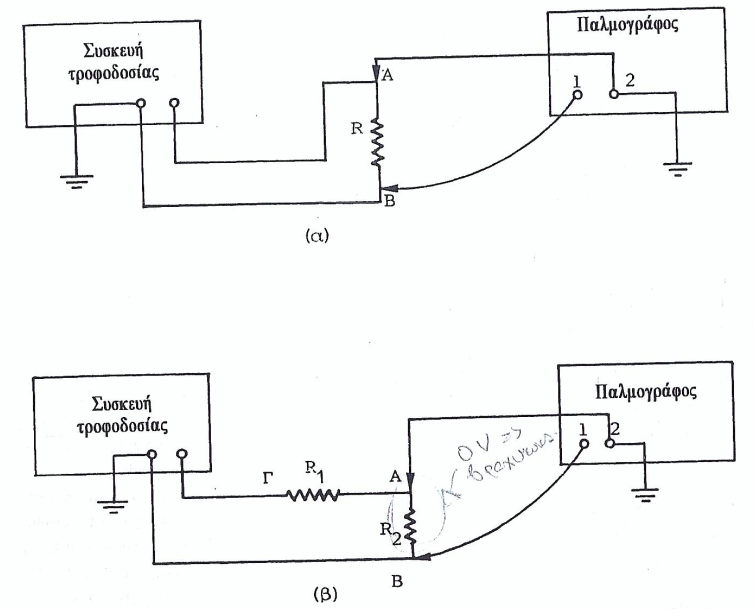
\includegraphics[width=\linewidth]{erwtisi64.png}
    \caption{}
    \label{erwtisi64}
\end{figure}
\emph{Σελ. 45-6}

\subsection{Ποιός είναι ο σκοπός εγκατάστασης μετασχηματιστών απομόνωσης?}
Αυτοί οι Μ/Τ ισχύος είναι συνήθως 1:1 με αγείωτο δευτερεύον, βρίσκονται εγκατεστημένοι κοντά στον πίνακα τροφοδοσίας και συνδέονται ανάμεσα από τον πίνακα και τις 
συσκευές (Σχήμα \ref{metasximatistisapomonwsis}). Αν ένα στοιχείο τάσης ακουμπήσει το μεταλλικό περίβλημα ενός οργάνου, τότε δεν διατρέχει κίνδυνο κάποιος που θα 
πιάσει το περίβλημα του οργάνου, γιατί δεν μπορεί να κλείσει κύκλωμα, αφού το δευτερεύον δεν είναι γειωμένο και δεν υπάρχει γαλβανική σύνδεση πρωτεύοντος με το 
δευτερεύον.  

\begin{figure}[h!]
    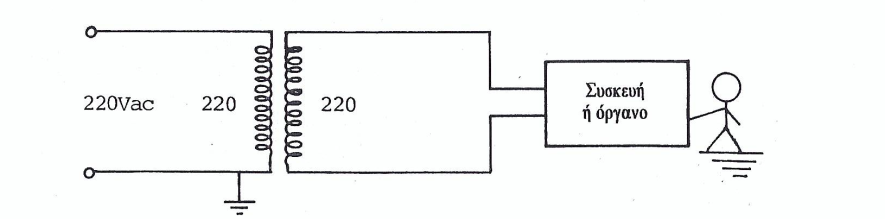
\includegraphics[width=\linewidth]{metasximatistisapomonwsis.png}
    \caption{Σύνδεση μετασχηματιστή απομόνωσης}
    \label{metasximatistisapomonwsis}
\end{figure}

\emph{Σελ. 47}

\subsection{Τι είναι οι διακόπτες διαφυγής?}
Ένα είδος προστασίας από την ηλεκτροπληξία. Υπάρχουν οι διακόπτες διαφυγής τάσης και έντασης ή αλλιώς διαφορικοί. 

O \textbf{διακόπτης διαφυγής τάσης} περιέχει ένα πηνίο τάσης. Όταν η τάση υπερβεί τα $50V$, έλκει τον οπλισμό του και διακόπτει όλες τις φάσεις και τον ουδέτερο σε
δέκατα του δευτερολέπτου.

O \textbf{διακόπτης διαφυγής έντασης} περιέχει έναν μεταχηματιστή και ένα πηνίο διακοπής/διαφυγής. Όταν δεν υπάρχει επαφή μεταξύ στοιχείου με τάση και του εξωτερικού
περιβλήματος, τα ρεύματα των αγωγών τροφοδοσίας είναι ίσα και δημιουργούν αντίθετα πολωμένα  μαγνητικά πεδία τα οποία αλληλοεξουδετερώνονται. Όταν υπάρχει σύνδεση μεταξύ 
στοιχείων και περιβλήματος, επάγεται τάση στο δευτερεύον του M/T, ενεργοποιείται το πηνίο διαφυγής και διακόπτεται το κύκλωμα σε λίγα δευτερόλεπτα.

\emph{Σελ. 48-50}

\subsection{Πώς προστατεύονται τα κυκλώματα? Πού πάνε τα μπαλόνια?}
Προστατεύονται με ασφάλειες και αυτόματους διακόπτες. Αν η ένταση του ρεύματος περάσει ένα όριο, διακόπτεται το κύκλωμα. Απαφεύγεται έτσι η πρόκληση πυρκαγιάς λόγω 
βραχυκυκλώματος και η καταστροφή των αγωγών των συσκευών.

\emph{Σελ. 50}
\subsection{Ποιά είναι η αρχή λειτουργίας αυτόματων διακοπτών?}
Έχουν ένα θερμικό και ένα μαγνητικό στοιχείο. 

Το θερμικό στοιχείο είναι ένα διμεταλλικό έλασμα το οποίο όταν θερμανθεί καθώς διαρέεται από ρεύμα λίγο περισσότερο από το κανονικό, παραμορφώνεται και προκαλεί
την διακοπή του κυκλώματος μετά από λίγο. 

Το μαγνητικό στοιχείο είναι ένα πηνίο με πυρήνα και έναν οπλισμό το οποίο διεγείρεται και διακόπτει αυτόματα το κύκλωμα όταν το ρεύμα γίνει πολύ μεγάλο.

\subsection{Ποιό σκοπό εξυπηρετούν οι αυτόματοι διακόπτες για έλλειψη τάσης και ποιό οι αυτόματοι για διαδοχή φάσεων?}

Οι \textbf{αυτόματοι διακόπτες για έλλειψη τάσης} διακόπτουν το κύκλωμα όταν η τάση πέσει κάτω από μια συγκεκριμένη τιμή 
(\foreignlanguage{english}{pretty self explanatory really}). 

Οι \textbf{αυτόματοι διακόπτες για διαδοχή φάσεων} διακόπτουν το κύκλωμα αν η τριφασική συνδεσμολογία έγινε λάθος και η διαδοχή των φάσεων είναι αντίθετη από την 
προβλεπόμενη. Εφαρμόζονται για την προστασία ηλεκτροκινητήρων οι οποίοι αλλάζουν φορά περιστροφής όταν αλλάζει η διαδοχή των φάσεων.

\emph{Σελ. 52}

\section{Ηλεκτρικός Θόρυβος}
\subsection{Τι λέγεται ηλεκτρικός θόρυβος?}
Είναι ανεπιθύματα σήματα που επηρεάζουν το κύκλωμα που μας ενδιαφέρει.

\emph{Σελ. 56}

\subsection{Ποιές είναι οι κύριες πηγές ηλεκτρικού θορύβου?}
\begin{itemize}
    \item Λάμπες φθορισμού και λάμπες νέον
    \item Ημιαγωγοί που χρησιμοποιούνται σαν διακόπτες (θυρίστορ και τρανζίστορ)
    \item Ηλεκτροκολλήσεις
    \item Λυχνίες θύρατρον
    \item Κάθε μορφής εκκένωση
    \item O \foreignlanguage{english}{Merzbow} (ειναι αντι\foreignlanguage{english}{SOS} αυτό δεν πέφτει ποτέ)
\end{itemize}

\emph{Σελ. 56}

\subsection{Ποιά είναι τα είδη σύζευξης ηλεκτρικού θορύβου?}
\begin{itemize}
    \item Ηλεκτροστατική ή χωρητική σύζευξη
    \item Μαγνητική ή επαγωγική
    \item Ηλεκτρομαγνητική
    \item Σύζευξη κοινής αντίστασης
\end{itemize}

\emph{Σελ. 56-7}

\subsection{Εξηγήστε τη φύση της ηλεκτροστατικής και της μαγνητικής \linebreak σύζευξης.}
Λέγονται και οι δύο μικρής απόστασης σύζευξης γιατί εξανεμίζονται όταν η απόσταση μεταξύ πηγής και δέκτη του θορύβου είναι μεγάλη.

Η \textbf{ηλεκτροστατική σύζευξη} οφείλεται στην χωρητικότητα μεταξύ πομπού και δέκτη και ο θόρυβος λόγω της ηλεκτροστατικής σύζευξης αυξάνεται όταν:
\begin{itemize}
    \item Αυξάνεται η συχνότητα
    \item Aυξάνεται η αντίσταση εισόδου του οργάνου
    \item Αυξάνεται η χωρητικότητα μεταξύ πηγής και δέκτη του θορύβου
\end{itemize}

Η \textbf{μαγνητική σύζευξη} οφείλεται στην τάση αλληλεπαγωγής μεταξύ πηγής και δέκτη, δηλαδή στις τάσεις που δημιουργούνται από επαγωγή λόγω μεταβολής μαγνητικών πεδίων. Ο θόρυβος αυξάνεται όταν:
\begin{itemize}
    \item Aυξάνεται η ένταση του μαγνητικού πεδίου
    \item Αυξάνεται ο εμπλεκόμενος με το μαγνητικό πεδίο βρόγχος του δέκτη
    \item Αυξάνεται η ταχύτητα μεταβολής του μαγνητικού πεδίου
    \item Μικραίνει η αντίσταση εισόδου
\end{itemize}

\emph{Σελ. 57-9}

\subsection{Εξηγήστε τη φύση της ηλεκτρομαγνητικής σύζευξης.}
Η ηλεκτρομαγνητική ακτινοβολία που εκπέμπεται από ραδιοφωνικούς και τηλεοπτικούς πομπούς μπορεί να δημιουργήσει θόρυβο κυρίως σε πολύ λεπτές μετρήσεις, ακόμα και σε 
περιπτώσεις που ο πομπός βρίσκεται πολύ μακριά από τον δέκτη (σύζευξη θορύβου μεγάλης απόστασης). Οι μη θωρακισμένοι αγωγοί δρούν σαν κεραίες ηλεκτρομαγνητικής 
ακτινοβολίας, οπότε τάση ηλεκτρομαγνητικού θορύβου αναπτύσσεται μεταξύ αυτών των αγωγών και της γης. (Κατατοπιστικότατο το ξέρω, τώρα που το ξαναβλέπω δεν είναι κακό)

\emph{Σελ. 60}

\subsection{Πότε εμφανίζεται σύζευξη κοινής αντίστασης?}
Εμφανίζεται όταν 2 ή και περισσότερα κυλώματα έχουν πολλούς κοινούς αγωγούς τροφοδοσίας και κατά συνέπεια τα ρεύματα των κυκλωμάτων περνούν από κοινές σύνθετες αντιστάσεις.

\emph{Σελ. 61}

\subsection{Να αναφερθούν τρόποι μείωσης του θορύβου.}
\begin{itemize}
    \item Τοποθέτηση των διατάξεων μετρήσεων μακριά από τις πηγές θορύβου (ηλεκτροστατική, μαγνητική)
    \item Το ¨στρίψιμο¨ των καλωδίων σε ευαίσθητες μετρητικές διατάξεις (ηλεκτροστατική, μαγνητική)
    \item Χρήση φίλτρων τροφοδοσίας αν υπάρχει θόρυβος που προέρχεται από την τροφοδοσία. Είναι χαμηλοπερατά φίλτρα που αφήνουν να περάσει η συχνότητα τροφοδοσίας και απορρίπτουν τον θόρυβο (κοινής αντίστασης)
    \item Χρήση θωράκισης, δηλαδή κάλυψης ενός αγωγού / στοιχείου με κάλυμα με συγκεκριμένες ηλεκτρομαγνητικές ιδιότητες που αποτρέπουν λήψη και εκπομπή ηλεκτρικού θορύβου (αγώγιμα πλέγματα για ηλεκτροστατική, σιδηρομαγνητικό υλικό για μαγνητική, αγώγιμο υλικό/στρώματα αγώγιμου και σιδηρομαγνητικού υλικού για ηλεκτρομαγνητική)
    \item Χρήση σωστών γειώσεων (υποθέτω για κοινή αντίστασης, μαγνητική, ηλεκτροστατική)
    \item Χρήση αγωγών μικρής αντίστασης (κοινής αντίστασης)
    \item Αποφυγή κοινών συνδέσεων (κοινής αντίστασης \foreignlanguage{english}{(duh)}) 
\end{itemize}
\emph{Σελ. 63-4}

\section{Όργανα με δείκτη}
\subsection{Εξηγήστε γιατί ένα όργανο με ανορθωτή παρουσιάζει αυξημένο σφάλμα όταν χρησιμοποιείται για μετρήσεις σε μη ημιτονοειδή ρεύματα.}
Οι ενδείξεις του οργάνου με ανορθωτή είναι σωστές μόνο όταν μετρούν ημιτονοειδή μεγέθη. Αν το μετρούμενο μέγεθος είναι παραμορφωμένο, περιέχει δηλαδή και άλλες αρμονικές
εκτός από τη θεμελιώδη, τότε η ένδειξη δεν ανταποκρίνεται στην ενδεικνύμενη τιμή του παραμορφωμένου μεγέθους. (τι σκατά σημαίνει ενδεικνύμενη τιμή)

\emph{Σελ. 96-7}

\section{Μέτρηση ισχύος και ενέργειας}
\subsection{Να περιγράψετε την αρχή λειτουργίας αντισταθμισμένων βαττόμετρων.}
Τα αντισταθμισμένα βαττόμετρα έχουν δύο πηνία τάσης, τα Π1 και Π2. Τα Π1 και Π2 είναι συνδεδεμένα σε σειρά μεταξύ τους και διαρρέονται με το ίδιο ρεύμα. Κατασκευαστικά, 
όμως, το Π2 είναι παράλληλα του πηνίου έντασης, αφαιρώντας το μαγνητικό πεδίο του Π2 από το πεδίο του πηνίου έντασης. Έτσι, στην ένδειξη του οργάνου δεν 
συμπεριλαμβάνεται η ισχύς που καταναλίσκεται στο πηνίο τάσης. Πρέπει όμως η σύνδεση του πηνίου τάσης να γίνει από την πλευρά της κατανάλωσης.

\emph{Σελ. 197-8}

\subsection{Να περιγράψετε τη μέτρηση ενεργού ισχύος με τη διάταξη \foreignlanguage{english}{Aron} σε τριφασικό σύστημα τριών αγωγών με συμμετρικές τάσεις.}
Η διάταξη στο σχήμα \ref{diataksiaron1} λέγεται διάταξη \foreignlanguage{english}{Aron}.

\begin{figure}[h!]
    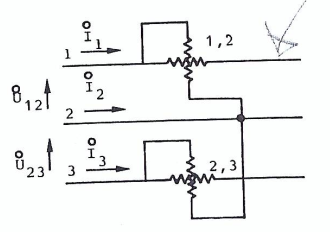
\includegraphics[width=10cm, height=10cm, keepaspectratio]{diataksiaron1.png}
    \caption{Διάταξη \foreignlanguage{english}{Aron}}
    \label{diataksiaron1}
\end{figure}
Οι τάσεις είναι συμμετρικές αλλά το ίδιο δεν ισχύει και για τις εντάσεις αν δεν έχουμε συμμετρικό φορτίο. 

Το πηνίο τάσης του βαττόμετρου 1,2 βρίσκεται υπό τάση $\mathring{U}_{1,2}$ ενώ το πηνίο έντασής του διαρρέεται από το ρεύμα $\mathring{I}_1$. Αντίστοιχα το πηνίο τάσης του 
βαττόμετρου 2,3 βρίσκεται υπό τάση $\mathring{U}_{2,3}$ ενώ το πηνίο έντασής του διαρρέεται από το ρεύμα $\mathring{I}_3$. Άρα οι ενδείξεις των βαττομέτρων θα είναι:

\begin{align*}
    P_{1,2} &= U_{1,2}I_1cos(30^\circ + \phi_1) \\
    P_{2,3} &= U_{2,3}I_3cos(30^\circ - \phi_3) 
    \intertext{Η συνολική ισχύς είναι το αλγεβρικό άθροισμα των ενδείξεων:}
    P =& P_{1,2} + P_{2,3}
    \intertext{Σε περίπτωση συμμετρικού φορτίου:}
    \mathring{I}_1 =& \mathring{I}_2 = \mathring{I}_3 \\
    \text{και αν } \phi_1 =& \phi_2 = \phi_3
    \intertext{τότε:}
    P_{1,2} =& 0 \\
    P_{2,3} = U_{32}I_3cos(60^\circ) =& U_{32}I_3\frac{\sqrt{3}}{2} = \sqrt{3}U_{32}I_3cos(60^\circ)
\end{align*}

Δηλαδή η συνολική ισχύς δίνεται από την ένδειξη του βαττομέτρου 2,3.

Αν $\phi_1 > 60^\circ$ η ένδειξη του βαττομέτρου 1,2 θα είναι αρνητική και αν $\phi_3 < -60^\circ$ η ένδειξη του βαττομέτρου 2,3 θα είναι αρνητική. Σε περίπτωση που ένα
βαττόμετρο έχει αρνητική ένδειξη, για να προσδιοριστεί η ένδειξη αντιστρέφεται η σύνδεση κάποιου πηνίου και η προκύπτουσα ένδειξη αφαιρείται από την
ένδειξη του άλλου βαττομέτρου.


\emph{Σελ. 202-3}

\subsection{Να περιγράψετε τη μέθοδο μέτρησης άεργου ισχύος σε τριφασικό σύστημα μετρήσεων με τρία βαττόμετρα.}

\begin{figure}[h!]
    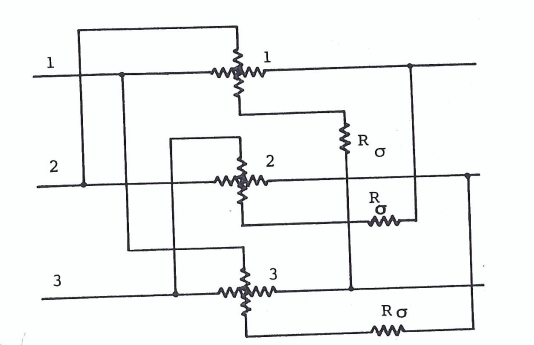
\includegraphics[width=10cm, height=10cm, keepaspectratio]{aei.png}
    \caption{Μετρητής άεργου ισχύος}
    \label{fig:4.3MAI}
\end{figure}

Η ένδειξη του βαττόμετρου 1 θα είναι: $U_{23}I_1\cos(90^\circ - \phi_1) = \sqrt{3}V_1I_1\sin(\phi_1) = \sqrt{3}Q_1$

Οι ενδείξεις των 2 και 3 αντίστοιχα:

\begin{align*}
    U_{31}I_2\cos(90^\circ - \phi_2)=\sqrt3Q_2 \\
    U_{12}I_3\cos(90^\circ - \phi_3)=\sqrt3Q_3
\end{align*}

Η τριφασική άεργος ισχύς είναι ίση με με το άθροισμα των ενδείξεων των βαττομέτρων διαιρεμένο δια $\sqrt{3}$. Σε περίπτωση συμμετρικού φορτίου, αρκεί ένα από τα τρία 
βαττόμετρα. Η άεργη ισχύς σε αυτή την περίπτωση θα είναι η ένδειξη του βαττομέτρου επί $\sqrt{3}$.

\emph{Σελ. 205-6}
\subsection{Εξηγήστε πως μπορεί να μετρηθεί ο συντελεστής ισχύος συμμετρικού τριφασικού κυκλώματος με τη διάταξη \foreignlanguage{english}{Aron}.}
Η μέτρηση του συντελεστή ισχύος σε συμμετρικά τριφασικά κυκλώματα μπορεί να γίνει άμεσα με τη χρήση δυο βαττομέτρων σε διάταξη \foreignlanguage{english}{Aron}. Λόγω
συμμετρίας:

\begin{align*}
    P_{1,2} + P_{2,3} = 3VIcos\phi \\
    \intertext{Εύκολα φαίνεται ότι:} \\
    P_{2,3} - P_{1,2} = \sqrt{3VIsin\phi}
    \intertext{Άρα:}
    tan\phi = \frac{\sqrt{3(P_{2,3} - P_{1,2})}}{P_{1,2} + P_{2,3}}
\end{align*}

Από την τελευταία εξίσωση υπολογίζεται η διαφορά φάσης $\phi$ και στη συνέχεια ο συντελεστής ισχύος $cos\phi$.

\emph{Σελ. 208}

% MEROS B MEROS B MEROS B MEROS B MEROS B MEROS B MEROS B MEROS B MEROS B MEROS B MEROS B MEROS B MEROS B MEROS B MEROS B MEROS B MEROS B MEROS B MEROS B MEROS B MEROS B MEROS B MEROS B
% MEROS B MEROS B MEROS B MEROS B MEROS B MEROS B MEROS B MEROS B MEROS B MEROS B MEROS B MEROS B MEROS B MEROS B MEROS B MEROS B MEROS B MEROS B MEROS B MEROS B MEROS B MEROS B MEROS B
% MEROS B MEROS B MEROS B MEROS B MEROS B MEROS B MEROS B MEROS B MEROS B MEROS B MEROS B MEROS B MEROS B MEROS B MEROS B MEROS B MEROS B MEROS B MEROS B MEROS B MEROS B MEROS B MEROS B

%\chapter{Μέρος Β}
\title{Μέρος Β}
\author{}
\date{}

\maketitle

\section{Εισαγωγή στα Συστήματα Μετρήσεων}
\subsection{Τι είναι μετατροπέας? Ποιοί είναι οι πιο διαδεδομένοι τύποι μετατροπών? Ποιά είναι η διαφορά μεταξύ ενός αισθητηρίου και ενός ανιχνευτή?}
Μετατροπέας λέγεται η διάταξη που απορροφά ενέργεια από ένα σύστημα και την μεταφέρει, αφού συνήθως τη μετατρέπει σε ενέργεια άλλης μορφής, σε ένα άλλο σύστημα. Κατατοπιστικότατο το ξέρω

Οι μετατροπείς που χρησιμοποιούνται για μετρήσεις είναι οι λεγόμενοι μετατροπείς εισόδου. Διεγείρονται από κάποια φυσική ποσότητα και δημιουργούν ένα σήμα εξόδου, συνήθως
ηλεκτρικό, το οποίο χρησιμοποιείται για την μέτρηση της αντίστοιχης φυσικής ποσότητας. Μετατροπείς εξόδου λέγονται οι μετατροπείς που μετατρέπουν ηλεκτρική ενέργεια 
σε ενέργεια άλλης μορφής, συνήθως μηχανική. Όταν χρησιμοποιούνται σε συστήματα ελέγχου λέγονται και ενεργοποιητές. Ένας μετατροπέας λέγεται ενεργός αν χρειάζεται 
για τη λειτουργία του μια εξωτερική πηγή ενέργειας. Ένας μετατροπέας λέγεται παθητικός αν δεν απαιτείται εξωτερική πηγή, αλλά η ενέργεια που απορροφάται από το μετρούμενο
σύστημα μετατρέπεται σε ενέργεια εξόδου (δηλαδή σε ενέργεια του σήματος που δημιουργείται σαν αποτέλεσμα του μετρούμενου μεγέθους). Οι πιο διαδεδομένοι τύποι μετατροπών 
είναι:

(Δεν ξέρω κατά πόσο αξίζει να μάθει κανείς αυτή τη λίστα τβη)

\begin{enumerate}
    \item Ηλεκτρομηχανικός τύπος 
    \item Τύπος ποτενσιόμετρου
    \item Τύπος διαφορικού μετασχηματιστή
    \item Τύπος πιεζοαντίστασης
    \item Φωτοηλεκτρικός τύπος
    \item Πιεζοηλεκτρικός τύπος 
    \item Θερμοηλεκτρικός τύπος
    \item Τύπος μεταβλητής ηλεκτρικής αντίστασης
    \item Τύπος θερμοδιαστολής
    \item Ημιαγωγικοί μετατροπείς θερμοκρασίας
    \item Χωρητικός τύπος 
    \item Επαγωγικός τύπος
    \item Τύπος ταλαντωτή
    \item Τύπος \foreignlanguage{english}{Hall} και μαγνητοαντίστασης
    \item Κουλ τύπος
\end{enumerate}

\textbf{Αισθητήριο} λέγεται μια διάταξη που χρησιμοποιείται για την μέτρηση ή ανίχνευση ενός φυσικού μεγέθους ενώ \textbf{ανιχνευτής} είναι μια διάταξη που 
χρησιμοποιείται για την ανίχνευση ενός φυσικού μεγέθους. (τα παράπονα στον Πετρίδη έτσι το έχει γράψει ο ίδιος)

\emph{Σελ. 271-3}
\subsection{Τι λέγεται ρύθμιση και τι ευαισθησία ενός συστήματος? Πότε λέμε ότι ένα σύστημα έχει γραμμικότητα μέτρησης και πότε ότι έχει γραμμική δυναμική συμπεριφορά?}
\scriptsize (Πήρε φόρα ο δικός σου)
\normalsize

\textbf{Ρύθμιση} ενός συστήματος μέτρησης λέγεται η διαδικασία κατά την οποία μεταβάλλεται αργά και με έναν γνωστό τρόπο η επιθυμητή είσοδος του συστήματος μέσα σε μια
περιοχή τιμών έτσι ώστε να καλυφθεί η περιοχή μέτρησης του συστήματος και να αντιστοιχηθεί σε κάθε τιμή της εξόδου μια τιμή της επιθυμητής εισόδου. Η γραμμική παράσταση
αυτής της αντιστοίχησης τιμών εισόδου και εξόδου λέγεται καμπύλη ρύθμισης.

\textbf{Ευαισθησία} λέγεται ο λόγος της μεταβολής της εξόδου προς τη μεταβολή της εισόδου στη μόνιμη κατάσταση λειτουργίας.

Ένα σύστημα έχει \textbf{γραμμικότητα μέτρησης} όταν η καμπύλη ρύθμισής του είναι μια ευθεία γραμμή.

Μπορεί ένα σύστημα να διέπεται από γραμμική διαφορική εξίσωση (\textbf{γραμμικότητα της δυναμικής του συστήματος}) αλλά να μην έχει γραμμικότητα μέτρησης.

\emph{Σελ. 292, 294}
\subsection{Τι γνωρίζετε για την υπερφόρτωση ενός μετρητή;}
Υπερφόρτιση ονομάζεται ο λόγος $\frac{\text{μέγιστη τιμή του μετρητή χωρίς να υποστεί βλάβη}}{\text{μέγιστη τιμή που μπορεί να μετρηθεί από μετρητή}}$ και αναφέρεται σε βλάβη. 
Μερικές φορές η υπερφόρτιση ορίζεται ως $\frac{\text{μέγιστη τιμή που δεν απορρυθμίζει το όργανο}}{\text{μέγιστη τιμή που μπορεί να μετρηθεί από μετρητή}}$ και αναφέρεται 
στην απορρύθμιση του οργάνου. Και οι δύο περιπτώσεις είναι στατικές υπερφορτίσεις. Υπάρχουν και δυναμικές υπερφορτίσεις που ορίζονται ανάλογα με τις στατικές, το μέγεθός
τους, όμως, αλλάζει ανάλογα με τη διάρκειά τους.


\emph{Σελ. 295}
\subsection{Ποιες συνθήκες πρέπει να πληρούνται ώστε η έξοδος ενός μετρητικού συστήματος να έχει το ίδιο σχήμα με την είσοδο?}
Αν η είσοδος αποτελείται από ένα φάσμα αρμονικών, η έξοδος θα έχει το ίδιο σχήμα με την είσοδο αν το κέρδος του συστήματος είναι σταθερό για
όλες τις αρμονικές της εισόδου και αν η διαφορά φάσης $\phi$ αυξάνει γραμμικά με τη συχνότητα. Τότε, η έξοδος θα είναι ίδιο σχήμα με την είσοδο,
αλλά χρονικά μετατοπισμένη. 

\emph{Σελ. 299}

\section{Μέτρηση Θέσης}
\subsection{Να υπολογιστεί η συνάρτηση μεταφοράς ενός ΓΜΔΜ ως προς την είσοδο διαμόρφωσης και να περιγραφεί η αρχή λειτουργίας ΓΜΔΜ.}
(Δεν ξέρω πόσο ρεαλιστικό είναι το να πέσει ο υπολογισμός της συνάρτησης μεταφοράς του ΓΜΔΜ σαν ερώτηση θεωρίας τβη, μπορεί να το βάλω για λόγους πληρότητας, αν δεν το έβαλα τότε
απλά βαριόμουν να το κάνω, σόρρυ)

Ο γραμμικός μεταβλητός διαφορικός μετασχηματιστής (ΓΜΔΜ) είναι ένας μετατροπέας διαφορικού μετασχηματιστή που παράγει στην έξοδό του ένα ηλεκτρικό σήμα το οποίο είναι ανάλογο με την 
μετατόπιση ή περιστροφή του οπλισμού. Ο ΓΜΔΜ έχει ένα πρωτεύον τύλιγμα και δύο δευτερεύοντα τα οποία συνδέονται σε σειρά αλλά έτσι ώστε οι τάσεις τους να αφαιρούνται. Η συχνότητα 
λειτουργίας των ΓΜΔΜ είναι $60Hz-20KHz$ και η τάση εισόδου είναι 3$V$ εώς 15$V$ συνήθως. Όταν ο οπλισμός είναι συμμετρικά τοποθετημένος η τάση εξόδου θεωρητικά είναι μηδενική (πρακτικά
πολύ μικρή). Η θέση αυτή ορίζεται σαν μηδενική θέση. Αν ο πυρήνας κινηθεί από τη μηδενική θέση ο συντελεστής ζέυξης του ενός δευτερεύοντος τυλίγματος αυξάνει ενώ του άλλου 
μειώνεται και έτσι εμφανίζεται μια τάση στην έξοδο η οποία είναι ανάλογη της μετατόπισης.

O ΓΜΔΜ λειτουργεί σαν ένας διαμορφωτής. Το φέρον σήμα είναι η τάση τροφοδοσίας και διαμορφωνεται κατά πλάτος από τη θέση του πυρήνα. οι συνηθισμένες τιμές της διαδρομής του πυρήνα είναι
μεταξύ ±$0.1mm$ εώς ±$75mm$.

Βασικά χαρακτηριστικά των ΓΜΔΜ: 

\begin{itemize}
    \item Γραμμικότητα μέτρησης
    \item Η ευαισθησία των των ΓΜΔΜ έιναι συνήθως μεταξύ $0,6$ και $30mV/0,001$ ίντσες. Ένας ΓΜΔΜ με μεγαλύτερη συχνότητα τάσης πρωτεύοντος και με μικρότερη διαδρομή του πυρήνα είναι πιο ευαίσθητος.
    \item Η δυναμική συμπεριφορά του ΓΜΔΜ περιορίζεται κυρίως από την συχνότητα της τάσης τροφοδοσίας του πρωτεύοντος. Για καλή αποδιαμόρφωση της τάσης εξόδου, θα πρέπει
        \newline$\frac{\text{συχνότητα τάσης του πρωτεύοντος}}{\text{μέγιστη συχνότητα κίνησης του πυρήνα}}\geq 10$
    \item Μεγάλη διακριτική ικανότητα
    \item Μεγάλη διάρκεια ζωής
    \item Αντοχή σε κραδασμούς και δεν απαιτείται συντήρηση
    \item Γαλβανική απομόνωση μεταξύ πρωτεύοντος και δευτερευόντων τυλιγμάτων
    \item Η έξοδος τους ειναι αρκετά ισχυρή και δεν χρειάζεται ενίσχυση
\end{itemize}

\begin{figure}[h!]
    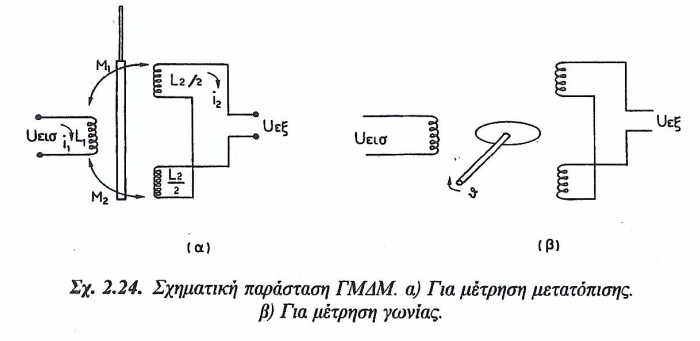
\includegraphics[width=\linewidth]{GMDM1.png}
    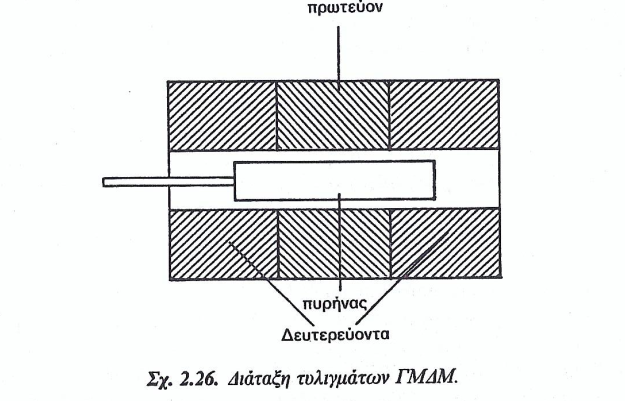
\includegraphics[width=\linewidth]{GMDM2.png}
\end{figure}
\emph{Σελ. 329-33}

\subsection{Περιγράψτε τη λειτουργία των οπτικών κωδικοποιητών μεταβολής.}
Οι οπτικοί κωδικοποιητές μεταβολής αποτελούνται από ένα δίσκο ο οποίος αποτελείται από διαδοχικούς διαφανείς και αδιαφανείς τομείς. Πολλές φορές φέρουν δόντια, ώστε οι
προεξοχές να έχουν τον ρόλο του αδιαφανούς και οι εσοχές τον ρόλο του διαφανούς τομέα. 

Ο κωδικοποιητής προσαρμόζεται σε έναν άξονα και ακολουθεί την περιστροφή του. Από τη μια πλευρά του κωδικοποιητή υπάρχει μια πηγή φωτός και από την άλλη ένας δέκτης φωτός.
Καθώς περιστρέφεται ο δίσκος εναλλάσονται οι διαφανείς και αδιαφανείς τομείς με αποτέλεσμα να παράγεται μια αλληλουχία παλμών το άθροισμα των οποίων 
δείχνει την γωνιακή θέση του άξονα. 

Η διακριτική ικανότητα ενός κωδικοποιητή εξαρτάται από τον αριθμό των παλμών (άρα των διαφανών και αδιαφανών τομέων του δίσκου). Πολλοί κωδικοποιητές χρησιμοποιούν 
και δεύτερο ζεύγος πομπού και δέκτη, δίνοντας παλμό για κάθε περιστροφή και τρίτο ζεύγος για προσδιορισμό της φοράς περιστροφής. 

Το μειονέκτημά τους είναι ότι δεν δείχνουν την απόλυτη θέση του άξονα, για αυτό απαιτούνται εξωτερικά κυκλώματα τα οποία μετρούν τους παλμούς και προσδιορίζουν τη θέση του
άξονα κάθε στιγμή.

\emph{Σελ. 333-4}


\section{Μέτρηση Ταχύτητας και Επιτάχυνσης}
\subsection{Περιγράψτε τη στροβοσκοπική μέθοδο μέτρησης περιστροφής ενός άξονα.}
Ας υποθέσουμε ότι ένας άξονας περιστρέφεται με ταχύτητα περιστροφής $n\;r/sec$ και ότι μία λάμπα που φωτίζει τον άξονα αναβοσβήνει με συχνότητα $f$. Αν υπάρχει κάποιο 
σημάδι επάνω στον άξονα θα φαίνεται ακίνητο στην περίπτωση που $n=kf$, με $k$ ακέραιο. Η μέτρηση γίνεται μεταβάλλοντας την συχνότητα $f$ έως ότου κάποιο σημάδι του άξονα
που ορίζεται για αυτό το σκοπό φανεί ακίνητο. Συνήθως η συχνότητα κυμαίνεται από $2$ έως $400 Hz$.

\emph{Σελ. 362-3}

\subsection{Περιγράψτε τη λειτουργία ταχογεννητριών.}
Οι ταχογεννήτριες παράγουν μια τάση ανάλογη της ταχύτητας περιστροφής του άξονά τους.

\begin{itemize}
    \item Οι ταχογεννήτριες \textbf{εναλλασσόμενου} ρεύματος είναι κινητήρες κλωβού δύο τυλιγμάτων. Το ένα τύλιγμα τροφοδοτείται με με εναλλασσόμενο ρεύμα. Λόγω της 
        περιστροφής του άξονα επάγεται στο άλλο τύλιγμα μια εναλλασσόμενη τάση με πλάτος ανάλογο της ταχύτητας περιστροφής. Η συχνότητα είναι ίση με τη συχνότητα 
        τροφοδοσίας και η φάση $180^\circ$ ή $0^\circ$, ανάλογα με τη φορά περιστροφής του άξονα. Η ευαισθησία αυτών των ταχόμετρων είναι μερικά βολτ ανά $1000\; rpm$.
        Η συχνότητα της φάσης τροφοδοσίας είναι $50-60$ ή $400Hz$. 
    \item Η ταχογεννήτρια \textbf{συνεχούς} ρεύματος είναι μια συνηθισμένη γεννήτρια συνεχούς ρεύματος η οποία έχει κατασκευαστικά καλή ακρίβεια και ευαισθησία. Η
        τάση εξόδου της είναι ανάλογη της ταχύτητας περιστροφής του άξονα και η πολικότητά της αλλάζει όταν αλλάζει η φορά του άξονα. Χρησιμοποιείται για ταχύτητες
        μέχρι μερικές χιλιάδες $rpm$. Έχουν ευαισθησία αρκετά βολτ ανά $1000\; rpm$.
\end{itemize}

\emph{Σελ. 364-5}

\subsection{Εξηγήστε πότε ένας μετατροπέας ταχύτητας λέγεται σχετικός και πότε απόλυτος.}

\begin{figure}[h!]
    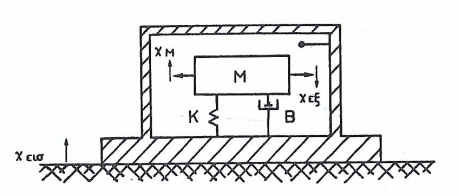
\includegraphics[width=\linewidth]{epitaxinsiometro.png}
    \caption{Βασικού τύπου επιταχυνσιόμετρο}
    \label{fig:5.1epitax}
\end{figure}

\begin{itemize}
    \item Ο \textbf{απόλυτος} μετατροπέας ταχύτητας αποτελείται από ένα επιταχυνσιόμετρο (Σχ. \ref{fig:5.1epitax}) και έναν μετατροπέα θέσης.
        Γίνεται χρήση της  αδρανειακής δύναμης που ασκείται στη μάζα Μ του επιταχυνσιόμετρου για τη μέτρηση της ταχύτητας.
    \item \textbf{Σχετικός} λέγεται ο μετατροπέας ταχύτητας που μετρά τη σχετική ταχύτητα ενός τμήματος του μετατροπέα ως προς ένα άλλο. (διαφωτιστικότατο)
\end{itemize}

\emph{Σελ. 369}

\subsection{Να υπολογίσετε τη συνάρτηση μεταφοράς ενός επιταχυνσιόμετρου βασικού τύπου (Σχήμα \ref{fig:5.1epitax}).}
(Και πάλι δεν ξέρω κατά πόσο πιθανό είναι να πέσει αυτό σαν ερώτηση θεωρίας)

Έστω $x_{\epsilon\iota\sigma}$ η μετατόπιση του περιβλήματος, $x_{\epsilon\xi}$ η μετατόπιση της μάζας Μ ως προς το περίβλημα και $x_M$
η μετατόπιση της Μ ως προς το σύστημα αναφοράς. Οι δυνάμεις που επενεργούν πάνω στη Μ όταν υπάρξει κάποια κίνηση της επιφάνειας στήριξης 
είναι:

Η αντίδραση του ελατηρίου:

\begin{align*}
    F_1 = Kx_{\epsilon\xi}
\end{align*}

και η αντίδραση του αποσβεστήρα:

\begin{align*}
    F_2 = B\frac{dx_{\epsilon\xi}}{dt}
\end{align*}

Το άθροισμα των δυνάμεων προκαλεί επιτάχυνση στο σώμα:

\begin{align*}
    Kx_{\epsilon\xi} + B\frac{dx_{\epsilon\xi}}{dt} = M\frac{d^2x_M}{dt^2}
\end{align*}

Ισχύει, όμως, ότι: 

\begin{align*}
    x_M = x_{\epsilon\iota\sigma} - x_{\epsilon\xi} \Rightarrow Kx_{\epsilon\xi} + B\frac{dx_{\epsilon\xi}}{dt} = M*\left(\frac{d^2x_{\epsilon\iota\sigma}}{dt^2} - \frac{d^2x_{\epsilon\xi}}{dt^2}\right)
\end{align*}

Παίρνοντας τον μετασχηματισμό \foreignlanguage{english}{Laplace} προκύπτει η συνάρτηση μεταφοράς του συστήματος:

\begin{align*}
    \frac{X_{\epsilon\xi}}{X_{\epsilon\iota\sigma}} = \frac{s^2M}{s^2M + sB + K} &= \frac{s^2}{s^2 + s\frac{B}{M} + \frac{K}{m}} \\
    \intertext{Θέτοντας:} \\ 
    \omega_n = \sqrt{\frac{K}{M}} \\
    \zeta = \frac{B}{2\sqrt{KM}} \\
    \intertext{έχουμε:}
    \frac{X_{\epsilon\xi}}{X_{\epsilon\iota\sigma}} = \frac{1}{s^2 + 2s\zeta\omega_n + \omega^2}
\end{align*}

Όπου $\omega_n$ η κυκλική φασική συχνότητα και $\zeta$ ο συντελεστής απόσβεσης του συστήματος. Η $\omega_n$ είναι η συχνότητα που θα ταλαντωνόταν το σύστημα αν $B=0$.

\emph{Σελ. 366-8}

\subsection{Να εξηγήστε γιατί το πιεζοηλεκτρικό επιταχυνσιόμετρο δεν μπορεί να μετρήσει σταθερή επιτάχυνση αφού υπολογίσετε την συνάρτηση μεταφοράς του.}
(\foreignlanguage{english}{Here we go again})

Η μάζα $M$ πιέζει τον πιεζοηλεκτρικό κρύσταλλο ο οποίος συνήθως βρίσκεται σε τάση ακόμα και για μηδενική επιτάχυνση (Σχήμα \ref{piezoepitaxinsiometro}), έτσι ώστε ο μετατροπέας να μπορεί να 
μετρήσει επιταχύνσεις και προς τις δύο φορές. Αν θεωρήσουμε την έξοδο του πιεζοηλεκτρικού κρυστάλλου την τάση $\upsilon$ και σαν είσοδο την μεταβολή $x$ της διάστασης 
του κρυστάλλου κατά την διεύθυνση μέτρησης, η συνάρτηση μεταφοράς θα είναι:

\begin{align*}
    \frac{V(s)}{X(s)} = \frac{K_k\tau s}{1 + \tau s} 
    \intertext{$\tau$ μια χρονική σταθερά, $K_k$ η ευαισθησία} 
\end{align*}

Η μεταβολή $x$ που ορίσαμε εδώ είναι η μεταβολή $X_{\epsilon \xi}$ (η οποία ορίζεται σε μια πολύ προηγούμενη εξίσωση στο βιβλίο, βλέπε Πετρίδη), οπότε προκύπτει (συνδυάζοντας με μια
άλλη εξίσωση που ορίστηκε πάλι πιο πριν μέσα στο βιβλίο, ξαναβλέπε Πετρίδη):

\begin{align*}
    \frac{V(s)}{\gamma (s)}  = & \frac{K_k\tau s}{(1 + \tau s)(s^2 + 2s\zeta \omega_n + \omega_n^2)} \\
    \intertext{με περιοχή συχνοτήτων λειτουργίας: } \\
    &\ \ \frac{3}{\tau} < \omega < \frac{\omega_n}{5} 
\end{align*}

Από την περιοχή συχνοτήτων φαίνεται ότι το πιεζοηλεκτρικό επιταχυνσιόμετρο δεν μπορεί να λειτουργήσει ούτε σε πολύ χαμηλές ούτε σε πολύ υψηλές συχνότητες. Επειδή 
έχουν μεγάλη φυσική συχνότητα $\omega_n$, τα καθιστά κατάλληλα για μετρήσεις επιταχύνσεων που περιέχουν υψηλές αρμονικές, άρα απότομες μεταβολές της επιτάχυνσης και άρα 
αδυνατούν στο να μετρήσουν σταθερή επιτάχυνση.

(Το γιατί τα πιεζοηλεκτρικά επιταχυνσιόμετρα δεν μπορούν να μετρήσουν σταθερή επιτάχυνση δεν το βρήκα στον Πετρίδη, οπότε κράτα μια επιφύλαξη για αυτό. Γιατί θεώρησε 
κάποιος ότι αυτή η ερώτηση ήταν καλή ιδέα να συμπεριληφθεί εδώ δεν θα καταλάβω ποτέ)

\begin{figure}[h!]
    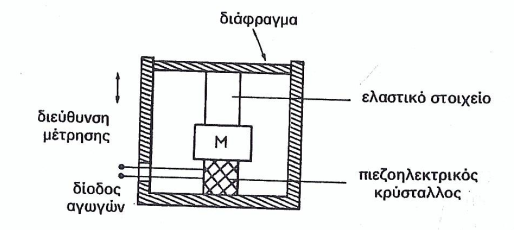
\includegraphics[width=\linewidth]{piezoepitaxinsiometro.png}
    \caption{Χαρακτηριστική κατασκευή πιεζοηλεκτρικού επιταχυνσιόμετρου}
    \label{piezoepitaxinsiometro}
\end{figure}

\emph{Σελ. 372-4}
\section{Μέτρηση Θερμοκρασίας}
\subsection{Να αναφέρετε και να εξηγήσετε πέντε βασικές ιδιότητες χρήσης θερμοζευγών.}
\begin{itemize}
    \item Αν τα δύο υλικά του θερμοζεύγους είναι ομοιογενή, η θερμοηλεκτρεγερτική του δύναμη δεν εξαρτάται από την θερμοκρασία κανενός σημείου εκτός από τις θερμοκρασίες των ενώσεων 1
        και 2.
    \item Ας υποθέσουμε ότι η θερμοκρασία της ένωσης 1 είναι $T_1$ και της 2 είναι $T_2$, όπως στο σχήμα \ref{fig:7.1thermo1} και η θερμοηλεκτρεγερτική δύναμη είναι Ε. 
        Έστω ότι καταστρέφεται η ένωση 1 και μεταξύ των υλικών Α και Β παρεμβάλλεται ένα άλλο υλικό Γ. Αν η θερμοκρασία των νέων ενώσεων ΒΓ και ΑΓ είναι $T_1$, τότε η 
        θερμοηλεκτρεγερτική δύναμη θα είναι ίση με Ε ακόμα και αν η θερμοκρασία των τμημάτων του Γ έξω από τις ενώσεις ΑΓ και ΒΓ είναι διαφορετική από την $T_1$.
        \begin{figure}[h!]
            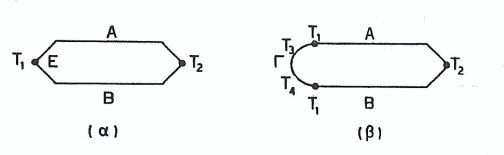
\includegraphics[width=\linewidth]{thermozevgi1.png}
            \caption{Θερμοστοιχείο με τρία υλικά και τρείς ενώσεις}
            \label{fig:7.1thermo1}
        \end{figure}
    \item Αν κοπεί ένα από τα δύο υλικά και παρεβληθεί ένα άλλο υλικό Γ, η ηλεκτρεγερτική δύναμη δεν μεταβάλλεται με την προϋπόθεση ότι οι ενώσεις π.χ. ΑΓ και ΓΑ έχουν την ίδια 
        θερμοκρασία $T_3$ ακόμη και αν η θερμοκρασία εκτός του Γ έξω από τις ενώσεις είναι διαφορετική από $T_3$. 
        \begin{figure}[h!]
            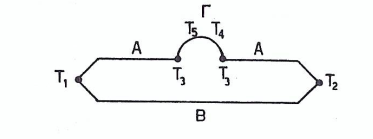
\includegraphics[width=\linewidth]{thermozevgi2.png}
            \caption{Θερμοστοιχείο με τρία υλικά και τέσσερεις ενώσεις}
            \label{fig:7.1thermo2}
        \end{figure}
    \item Έστω ένα θερμοζεύγος παράγει μια θερμοηλεκτρεγερτική δύναμη $E_1$ όταν οι θερμοκρασίες των ενώσεων 1 και 2 είναι $T_1$ και $T_2$ αντίστοιχα ($Τ_2 > Τ_1$). Όταν οι 
        θερμοκρασίες των ενώσεων 1 και 2 είναι $T_2$ και $T_3$ αντίστοιχα ($Τ_3 > Τ_2$), έστω η παραγόμενη θερμοηλεκτρεγερτική δύναμη είναι $E_2$. Αν οι θερμοκρασίες των 
        ενώσεων 1 και 2 είναι $T_1$ και $T_3$ αντίστοιχα, η θερμοηλεκτρεγερτική δύναμη που θα παραχθεί θα είναι $E_1+E_2$. \item Αν η θερμοηλεκτρεγερτική δύναμη 
        μεταξύ των υλικών Α και Γ είναι $E_{A\Gamma}$ και μεταξύ των υλικών Γ και Β είναι $E_{\Gamma B}$ η θερμοηλεκτρεγερτική δύναμη των υλικών Α και Β θα είναι 
        $E_{A\Gamma} + E_{\Gamma B}$.
\end{itemize}

\emph{Σελ. 422-3}

\subsection{Να αναφέρετε δύο τρόπους σύνδεσης ενός θερμοστοιχείου με όργανο και να εξηγήσετε τη λειτουργία τους.}
Για την μέτρηση της ηλεκτρεγερτικής δύναμης $E$ και την αντιστοίχησή της σε κάποια θερμοκρασία χρησιμοποιούνται όργανα μέτρησης τάσης. Τα όργανα αυτά είναι σε 
κάποια απόσταση από την ένωση του θερμοζεύγους (Σχήμα \ref{thermozevgi3}). Για να μετρηθεί σωστά η $E$ με τις συνδέσεις των σχημάτων \ref{thermozevgi3}α και 
\ref{thermozevgi3}γ πρέπει οι ακροδέκτες του οργάνου να βρίσκονται στην ίδια θερμοκρασία. Για να μετρηθεί σωστά η $E$ με την σύνδεση \ref{thermozevgi3}β πρέπει οι 
ενώσεις 2 και 3 του θερμοζεύγους με τα καλώδια επέκτασης να βρίσκονται στην ίδια θερμοκρασία.  Στο σχήμα \ref{thermozevgi3}α η ένωση $2$ και στο σχήμα 
\ref{thermozevgi3}β οι ενώσεις $2$ και $3$ μπορούν να κρατηθούν σε σταθερές και επιθυμητές θερμοκρασίες με ένα μπάνιο (σήκω και κάνε ένα τώρα, ζέχνεις). 
Οι ενώσεις αυτές λέγονται ενώσεις αναφοράς και η θερμοκρασία τους θερμοκρασία αναφοράς. 

\begin{figure}[h!]
    \includegraphics[height=2in]{thermozevgi3.png}
    \caption{Συνδέσεις θερμοστεοιχείου με όργανο}
    \label{thermozevgi3}
\end{figure}

(Ειλικρινά δεν είναι και η καλύτερη απάντηση αυτή αλλά \foreignlanguage{english}{I tried my best})

\emph{Σελ. 423-4}

\subsection{Τι είναι η ηλεκτρική αντιστάθμιση θερμκρασίας?}
Μπορεί να επιτευχθεί σταθερή διατήρηση της θερμοκρασίας στην ένωση αναφοράς ενός θερμοζεύγους (για μετρήσεις ακριβείας) με τη διάταξη που ονομάζεται ηλεκτρική αντιστάθμιση
θερμοκρασίας. Υπάρχει μια γέφυρα (Σχήμα \ref{antistathmisithermokrasias}) στην οποία η αντίσταση $R_\theta$ μεταβάλλεται με την θερμοκρασία. Η αντίσταση αυτή και οι ενώσεις αναφοράς βρίσκονται σε πολύ
καλή θερμική επαφή έτσι ώστε να έχουν την ίδια θερμοκρασία. Όταν η θερμοκρασία στις ενώσεις αναφοράς είναι $0^\circ C$, η τάση στα άκρα της γέφυρας είναι μηδενική, ενώ
με τη μεταβολή της θερμοκρασίας μεταβάλλεται η τιμή της αντίστασης και η γέφυρα δεν ισορροπεί πλέον, οπότε εμφανίζεται μια τάση στα άκρα της. Έτσι, η τάση στην έξοδο ΑΒ
είναι ίση με την θερμοηλεκτρεγερτική δύναμη του θερμοζεύγους όταν η θερμοκρασία αναφοράς είναι $0^\circ C$. Η διάταξη ηλεκτρικής αντιστάθμισης έχει συνήθως πολύ μεγάλη
διάρκεια ζωής και είναι μικρή (τυπικό βάρος είναι λίγες δεκάδες γραμμάρια).

\begin{figure}[h!]
    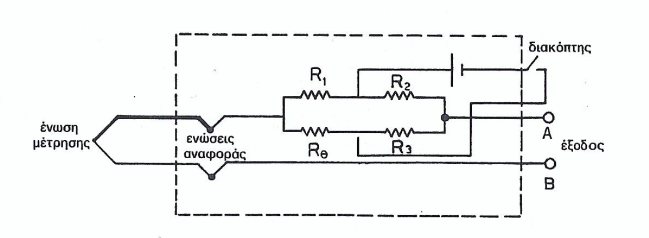
\includegraphics[width=\linewidth]{antistathmisithermokrasias.png}
    \caption{Ηλεκτρική αντιστάθμιση θερμοκρασίας αναφοράς}
    \label{antistathmisithermokrasias}
\end{figure}

\emph{Σελ. 426-7}
\subsection{Περιγράψτε τους δύο τρόπους γραμμικοποίησης ενός θερμίστορ.}
Τα θερμίστορ κατασκευάζονται από οξειδια μετάλλων και η αντίστασή τους μειώνεται καθώς η θερμοκρασία αυξάνει. 

Ένας τρόπος γραμμικοποίησης φαίνεται στο σχήμα \ref{thermistor}α. Οι τάσεις $V1$ και $V2$ εμφανίζουν γραμμική μεταβολή στο μέσον της περιοχής μέτρησης. Η $V1$ έχει 
θετική κλίση και η $V2$ αρνητική. Η διάταξη αυτή χρησιμοποιείται κυρίως σαν διαιρέτης τάσης που εξαρτάται από τη θερμοκρασία, δηλαδή η $V2$ εξαρτάται γραμμικά από 
τη θερμοκρασία. Η διάταξη στο σχήμα \ref{thermistor}β χρησιμοποείται σαν αντίσταση που μεταβάλλεται γραμμικά με τη θερμοκρασία.

(Πώς γίνεται μια ερώτηση θεωρίας να έχει ως απάντηση δύο σχήματα? Πιθανό αλλά μου φαίνεται λίγο περίεργο)

\begin{figure}[h!]
    \includegraphics[width=\linewidth]{thermistor.png}
    \caption{Δύο τρόποι γραμμικοποίησης ενός θερμίστορ}
    \label{thermistor}
\end{figure}

\emph{Σελ. 432}

\subsection{Τι γνωρίζετε για του ημιαγωγικούς μετατροπείς θερμοκρασίας;}
Οι πιο σημαντικοί ημιαγωγικοί μετατροπείς θερμοκρασίας είναι αντιστάσεις, δίοδοι και ολοκληρωμένα κυκλώματα.

\begin{itemize}
    \item Οι \textbf{ημιαγωγικές αντιστάσεις} έχουν θετικό συντελεστή θερμοκρασίας, συνήθως $0,8\%$ της πλήρους κλίμακας ανά $^{\circ}C$. Η γραμμικότητά τους είναι καλή.
        Οι τιμές των ημιαγωγικών αντιστάσεων σε κανονική θερμοκρασία ποικίλλει από δεκάδες $Ohm$ σε δεκάδες $K\Omega$. Μπορούν να χρησιμοποιηθούν σε γέφυρα όπως τα
        $RTD$ και τα θερμίστορ.
    \item Στις \textbf{διόδους} η μεταβολή της τάσης προς θερμοκρασία είναι $-2,3mV/^{\circ}C$ για ενώσεις πυριτίου και $-2,1mV/^{\circ}C$ για ενώσεις γερμανίου (όσο 
        αυξάνεται η θερμοκρασία μειώνεται η τάση). Η εξάρτηση της τάσης από τη θερμοκρασία σε διόδους και τρανζίστορ χρησιμοποιείται για κατασκευή μετατροπέων θερμότητας
        με γρήγορη απόκριση.
    \item Υπάρχουν \textbf{ολοκληρωμένα κυκλώματα} που λειτουργούν σαν πηγές ρεύματος των οποίων η ένταση εξαρτάται από τη θερμοκρασία. Χρησιμοποιούνται για γραμμικούς
        μετατροπείς θερμοκρασίας οι οποίοι είναι πολύ εύκολοι στη χρήση.
\end{itemize}

\emph{Σελ. 433}

\subsection{Ένα θερμοζεύγος (Σχήμα \ref{thermikozevgos})έχει τη μία ένωση σε $25^{\circ} C$ και την άλλη σε $T_1$. Αν η μετρούμενη τάση είναι $E_1=3,991mV$ 
ποιά είναι η τάση στο άκρο $T_1$?}
Μεταξύ $T_1$ και $T_2$ υπάρχει θερμοηλεκτρεργετική δύναμη $E_1 = 3,991 mV$. Αν θεωρήσουμε $T_3 = 0^{\circ}C$ μεταξύ $T_2$ και $T_3$ βλέπουμε από τον πίνακα 
\ref{82pinakas} ότι θα έχουμε $E_2 = 1,277mV$, αφού $T_2 - T_3 = 25^{\circ}C$. Άρα μεταξύ $T_1$ και $T_3$ θα έχουμε $E = E_1 + E_2 = 5,268mV$ (4η ιδιότητα 
θερμοζευγών, βλ. 8.1), άρα από τον πίνακα \ref{82pinakas} $T_1 = 100^{\circ}C$.

\begin{figure}[h!]
    \centering
    \begin{subfigure}[b]{0.4\linewidth}
        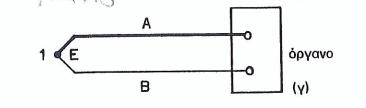
\includegraphics[width=\linewidth]{thermikozevgos.png}
        \caption{Σύνδεση θερμοστοιχείου με όργανο}
        \label{thermikozevgos}
    \end{subfigure}
    \begin{subfigure}[b]{0.4\linewidth}
        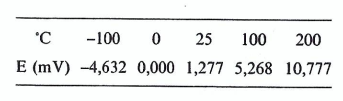
\includegraphics[width=\linewidth]{82pinakas.png}
        \caption{Πίνακας θερμοκρασιών}
        \label{82pinakas}
    \end{subfigure}
    \caption{}
\end{figure}

\emph{Ασκ. 2 Σελ. 434, τρόπος λύσης Σελ. 424}

\subsection{Η μεταβολή αντίστασης με τη θερμοκρασία ενός $RTD$ από λευκόχρυσο για την περιοχή $0-630^{\circ}C$ περιγράφεται από την εξίσωση $R_t=R_o(1+0.00398T - 0.588*10^{-6}T^2)$
όπου $R_t$ και  $R_o$ είναι οι αντιστάσεις του $RTD$ στις θερμοκρασίες $T$ και $0$ αντίστοιχα. Να υπολογισθεί το σφάλμα γραμμικότητας μέτρησης της θερμοκρασίας στις θερμοκρασίες 
$200^{\circ}C$ και $500^{\circ}C$.}

(Υποθετική λύση) Έστω ότι λείπει ο μη γραμμικός όρος $-0.588*10^{-6}T^2$. Τότε στους $200^{\circ}C$ θα είναι:

\begin{align*}
    & R_{200linear} = R_o(1+0.00398*200)=1.76R_o \\
    \text{eνώ }&R_{200real} = 1.75648R_o \text{ που είναι μια διαφορά } 2.224925\% \\
     \intertext{Ομοίως:} &\\
    &  R_{500linear} = 2.99R_o \\
    & R_{500real} = 2.843R_o \text{ που είναι μια διαφορά τάξης } 5.04029\% 
\end{align*} 

\emph{Ασκ. 9 Σελ. 435}

\section{Συστήματα προσαρμογής}
\subsection{Ένας μονοπολικός μετατροπέας έχει εύρος μετατροπής $0-25V$. Για έξοδο των $12\; bits$ να υπολογισθεί η διακριτική ικανότητα του μετατροπέα για την περίπτωση 
του δυαδικού κώδικα και του $BCD$.}
Για την περίπτωση του δυαδικού κώδικα αν ο μετατροπέας έχει $n\; bits$, η έξοδος μπορεί να πάρει $N=2^n$ διαφορετικές τιμές. Έτσι αν το εύρος μετατροπής είναι Ε, η διακριτική
ικανότητα του μετατροπέα θα είναι $E/2^n$. Στον κώδικα $BCD$ κάθε ψηφίο σε έναν δεκαδικό αριθμό παριστάνεται από $4\; bits$. Μετατροπείς που χρησιμοποιούν $BCD$ 
έχουν αριθμό $bits$ που έιναι πολλαπλάσιο του 4. Αν ο μετατροπέας $BCD$ έχει $4\; bits$, η έξοδος μπορεί να πάρει $N=10$ διαφορετικές τιμές ενώ αν έχει $8\; bits$ η
έξοδος μπορεί να πάρει $N=100$ διαφορετικές τιμές, άρα η διακριτική ικανότητα για $12\; bits$ θα είναι $\Delta E_{BCD}=\frac{2.5}{1000}$.

\emph{Σελ. 455-6}

\subsection{Ποιά τα πλεονεκτήματα μετάδοσης σήματος με ένταση ρεύματος $4-20mA$? Τι σημαίνει σφάλμα κλίμακας σε έναν $A/D$ μετατροπέα?}
Ας θεωρήσουμε για παράδειγμα ότι η έξοδος κάποιου μετατροπέα μεταβάλλεται από $0$ έως $10V$. Για να χρησιμοποιηθεί μετάδοση $4-20 mA$ πρέπει να γίνει μετατροπή της 
τάσης σε ρεύμα έτσι ώστε $0V$ να αντιστοιχούν σε $4 mA$ και $10V$ να αντιστοιχούν σε $20 mA$.Τα κύρια πλεονεκτήματα αυτού του τρόπου μετάδοσης είναι:

\begin{itemize}
    \item τα $4mA$ παριστούν το μηδέν ενώ τα $0mA$ τη διακοπή του κυκλώματος
    \item η χρήση ρεύματος μειώνει την επίδραση των θορύβων
\end{itemize}

Το σφάλμα κλίμακας σημαίνει ότι η μέγιστη έξοδος δεν εμφανίζεται για την αντίστοιχη μέγιστη τιμή εισόδου. Με άλλα λόγια, η διαφορά της εισόδου κατά τη μεταβολή της 
εξόδου από $1110$ σε $1111$ με την είσοδο κατά τη μεταβολή της εξόδου από $0000$ σε $0001$ δεν ισούται με $E_{fs}-2LSB$. Το σφάλμα κλίμακας δίνεται σαν το ποσοστό 
της πλήρους κλίμακας.

\emph{Σελ. 453, 461}

\subsection{Για τη μετατροπή αναλογικού σήματος $7V$ χρησιμοποιείται ένας μετατροπέας $A/D$ κλιμακωτής ανόδου και ένας μετατροπέας $A/D$ διαδοχικών προσεγγίσεων. Και οι δύο έχουν έξοδο 
$10\; bit$, $D/A$ με χρόνο μετατροπής $2\mu s$ και το εύρος μετατροπής τους είναι $0-12V$. Να υπολογισθεί ο χρόνος μετατροπής και των δύο μετατροπέων $A/D$ αν θεωρήσουμε ότι ο χρόνος
μετατροπής τους εξαρτάται μόνο από τον χρόνο μετατροπής του $D/A$.}
    
\begin{itemize}
    \item Για την κλιμακωτή άνοδο έχουμε ότι $LSB = \frac{12}{2^{10}} = 11.71875mV$ kai εφόσον η έξοδος του $D/A$ θα αυξάνει συνεχώς κατά την τιμή ενός $LSB$ μέχρι να φτάσει τα $7V$, 
        θα έχουμε $x = |\frac{7000}{LSB}| = 598$ επαναλήψεις, άρα ο χρόνος μετατροπής θα είναι $598*2\mu s = 1.169ms$
    \item Η τεχνική των διαδοχικών προσεγγίσεων απαιτεί όσες μετατροπές όσα τα $bits$ στην έξοδο του $A/D$, άρα $x = n = 10$ kai $\Delta t = x * 2\mu s = 20\mu s$
\end{itemize}
\emph{Σελ. 462-3}

\subsection{Να περιγραφεί η αρχή λειτουργίας ενός μετατροπέα $A/D$ διαδοχικών μετατροπών. (Σχ. \ref{addiadoxikwn})}
Η τεχνική διαδοχικών προσεγγίσεων απαιτεί τόσες μετατροπές στον μετατροπέα $D/A$ όσος είναι ο αριθμός των $bits$ της εξόδου στον $A/D$. Μόλις δοθεί το σήμα εισόδου, το 
$MSB$ του καταχωρητή γίνεται 1, ανώ τα υπόλοιπα $bits$ είναι μηδενικά. Έτσι, έξοδος του $D/A$ θα είναι το μισό του εύρους μετατροπής. Αν η αναλογική είσοδος του $A/D$ 
είναι μεγαλύτερη από την έξοδο του $D/A$, μένει το 1 στο $MSB$ του καταχωρητή, αλλιώς γίνεται 0. Στη συνέχεια, το $n-2\;bit$ του καταχωρητή γίνεται 1 ενώ το $n-1\;bit$ (εδώ το $MSB$)
διατηρεί την προηγούμενη τιμή του. Η νέα έξοδος θα είναι $3/4$ του εύρους μετατροπής αν $MSB=1$ ή $1/4$ του εύρους μετατροπής αν $MSB=0$. Αν η αναλογική είσοδος του
$A/D$ είναι μεγαλύτερη της εξόδου του $D/A$, τότε παραμένει το 1, αλλιώς γίνεται 0. Η ίδια διαδικασία επναλαμβάνεται για όλα τα υπόλοιπα $bits$. Όταν γίνει αυτή η διαδικασία 
δίνεται το σήμα ΤΜ (τέλους μετατροπής). Το πλεονέκτημα αυτού του μετατροπέα είναι ο μικρός χρόνος μετατροπής.

\begin{figure}[h!]
    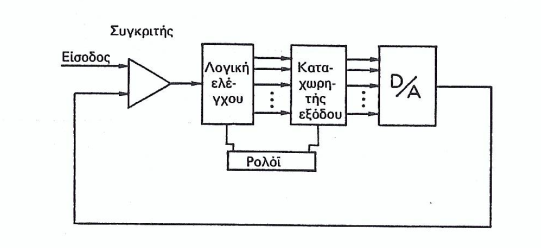
\includegraphics[width=\linewidth]{metatropeasdiadoxikwnproseggisewn.png}
    \caption{Μετατροπέας $A/D$ διαδοχικών προσεγγίσεων σε απλή μορφή}
    \label{addiadoxikwn}
\end{figure}

\subsection{Περιγράψτε την λειτουργία του μετατροπέα $A/D$ διπλής 
ολοκλήρωσης. (Σχ. \ref{addiplisolok})}
%\newpage

\begin{figure}[h!]
    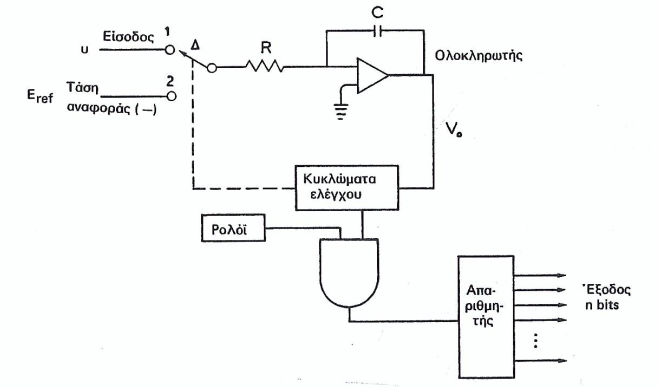
\includegraphics[width=\linewidth]{AD2olok.png}
    \caption{Μετατροπέας $A/D$ διπλής ολοκλήρωσης απλής μορφής}
    \label{addiplisolok}
\end{figure}
Μόλις δοθεί το ΣΕ ο διακόπτης Δ πηγαίνει στη θέση 1. Η ολοκλήρωση διαρκεί για ένα χρονικό διάστημα Τ το οποίο μετριέται στον απαριθμητή και αντιστοιχεί σε $N_1$. $N_1$ είναι το μέγιστο 
περιεχόμενο του απαριθμητή. Μετά την παρέλευση του χρονικού διαστήματος Τ η έξοδος του ολοκληρωτή είναι: 

\begin{align*}
    V_o=-\frac{1}{RC}\int^{T}_{0} \upsilon dt=-\frac{\upsilon}{RC}T
\end{align*}

Στη συνέχεια ο διακόπτης Δ πηγαίνει στη θέση 2 και ο απαριθμητής μηδενίζεται. Έτσι ο απαριθμητής αρχίζει να μετράει από το μηδέν ενώ η έξοδος του ολοκληρωτή μειώνεται γραμμικά δεδομένου
ότι η είσοδός του είναι η αρνητική τάση αναφοράς. Όταν μηδενισθεί η έξοδος του ολοκληρωτή τελειώνει η μετατροπή. Το περιεχόμενο $N_2$ του απαριθμητή έιναι η ψηφιακή παράσταση της 
αναλογικής εισόδου. Η έξοδος του ολοκληρωτή είναι: 

\begin{align*}
    V_o = -\frac{\upsilon}{RC}T + \frac{1}{RC} \int^t_0 E_{ref}dt = - \frac{\upsilon}{RC}T + \frac{E_{ref}}{RC}t
\end{align*}

Όταν $V_o = 0$, τότε $t=\frac{\upsilon}{E_{ref}}T$ και $N_2=\frac{\upsilon}{E_{ref}}N_1$.

Σε αυτόν τον μετατροπέα οι μεταβολές με το χρόνο ή την θερμοκρασία των $R$, $C$ και της συχνότητας του ρολογιού δεν παίζουν ρόλο (εκτός αν αλλάξουν κατά τη διάρκεια μιας μετατροπής).
Η γραμμικότητα αυτού του μετροπέα είναι πολύ καλή, αλλά ο χρόνος μετατροπής είναι πολύ μεγάλος.

\emph{Σελ. 464-5}

\subsection{Πρόκειται να σχεδιαστεί ένα σύστημα μετατροπής $A/D$ με εύρος μετατροπής $-10V$ εώς $10V$ και $10\;bits$ που μπορεί να μετατρέπει αναλογικά σήματα με μέγιστη ταχύτητα $5kHz$
και ταχύτητα δειγματοληψίας $100\; samples/sec$. Να υπολογισθεί ο απαιτούμενος χρόνος συγκράτησης του $S/H$ και ο χρόνος μετατροπής του μετατροπέα $A/D$.}
\begin{align*}
    \Delta E = \frac{20}{2^{10}} = 19,53125*10^{-3}\;& \text{(δεν καταλαβαίνω γιατί αυτό είναι απαραίτητο)} \\
    \intertext{Χρόνος συγκράτησης:} \\
    \Delta t &= \frac{1}{2\pi5*10^3*2^{10}} \\ 
    \intertext{Χρόνος μετατροπής:}
    f_{conv} = \frac{100}{100^{-3}} &= 100kHz \Rightarrow \Delta t = \frac{1}{100*10^3} = 10^{-5}s
\end{align*}

\emph{Σελ. 467}

\subsection{Για έναν μονοπολικό μετατροπέα $A/D$ με $n\; bits$ και κύκλωμα συγκράτησης $S/H$ να υπολογίσετε τη μέγιστη συχνότητα που μπορεί να μετατρέψει χωρίς σφάλμα.}
Έστω πλάτος σήματος $\text{E}_{FS}$. Αν $\Delta E$ το αναλογικό σήμα που αντιπροσωπεύει ένα $LSB$ μετατροπής, τότε η μέγιστη επιτρεπτή μεταβολή του σήματος προς μετατροπή είναι 
$\frac{\Delta \text{E}}{2}$. Αν το σήμα εισόδου είναι ημιτονοειδές με πλάτος $\text{Ε}_{FS}$ και φάση του είναι $2\pi ft$, ο μέγιστος ρυθμός μεταβολής εμφανίζεται για $t = 0$ και είναι $2\pi f E_{FS}$.
Τότε, $2 * 2 \pi fE_{FS} \leq \Delta E$. Αφού έχουμε μονοπολικό μετατροπέα, $\Delta E = \frac{E_{FS}}{2^n}$ άρα έχουμε ότι $f \leq \frac{1}{4\pi2^n\Delta t}$ όπου $\Delta t$ ο χρόνος
συγκράτησης του κυκλώματος $S/H$.


\emph{Σελ. 467}

\subsection{Να εξηγήσετε τη χρησιμότητα ενός κυκλώματος συγκράτησης $(S/H)$ και του πολυπλέκτη.}
Κύκλωμα συγκράτησης: Για να γίνει σωστή η μετατροπή $A/D$, η αναλογική είσοδος δεν πρέπει να μεταβάλλεται πάνω από το όριο μεταβολής $1/2LSB$. Παρατηρούμε ότι κανονικά,
ακόμα και πολύ χαμηλές συχνότητες θα μπορούσαν να μετατραπούν μόνο από τους γρηγορότερους μετατροπείς. Για να ξεπερασθεί αυτό το πρόβλημα, η είσοδος πρέπει να κρατηθεί σταθερή. Για
αυτό το λόγο χρησιμοποιούνται τα κυκλώματα συγκράτησης, τα οποία κρατούν την έξοδό τους σταθερή (είσοδος του μετατροπέα) όταν λαβουν εντολή συγκράτησης. Υπάρχει, 
βέβαια χρόνος συγκράτησης, όμως είναι πολύ μικρός σε σχέση με το χρόνο μετατροπής, επτρέποντας την μετατροπή υψηλότερων συχνοτήτων.

Πολυπλέκτης: Έαν θέλουμε να μετατρέψουμε πολλά αναλογικά σήματα σε ψηφιακά, θα μπορούσαμε να χρησιμοποιήσουμε έναν μετατροπέα $A/D$ γαι κάθε σήμα. Όμως αυτή η λύση είναι
πολύ ακριβή, για αυτό τοποθετούμε έναν μετατροπέα $A/D$ μετά από έναν πολυπλέκτη. Η μετατροπή των σημάτων γίνεται διαδοχικά, με την προϋπόθεση ότι η ταχύτητα δειγματοληψίας που
απαιτείται για κάθε σήμα είναι τέτοια, ώστε να προλαβαίνει να ανταποκρίνεται ο μετατροπέας $A/D$.

Όταν έρθει η εντολή εκκίνησης στον πολυπλέκτη, η τιμή στην είσοδο των διευθύνσεων τη στιγμή εκείνη καθορίζει ποιά αναλογική είσοδος θα περάσει στην έξοδο, ενώ οι 
υπόλοιπες αναλογικές εισόδοι θα απομονωθούν.

\emph{Σελ. 467-8}

\subsection{Περιγράψτε την αρχή λειτουργίας ενός μετατροπέα $D/A$ ρεύματος.}
Οι μετατροπείς $D/A$ ρεύματος λειτουργούν μέσω κυκλωμάτων που δημιουργούν ρεύματα $i$,$i/2$,$i/4$ κλπ. τα οποία αθροίζονται στην έξοδο (Σχήμα \ref{DArevmatos}). Αν μία δίοδος συνδεθεί σε λογικό 0, άγει και 
βραχυκυκλώνει το αντίστοιχο τρανζίστορ από το οποίο δεν περνάει ρεύμα. Αν μία δίοδος συνδεθεί σε λογικό 1, δεν άγει και το ρεύμα περνάει από το αντίστοιχο τρανζίστορ. Έτσι, το 
ρεύμα εξοδου εξαρτάται από την ψηφιακή είσοδο και η τιμή του καθορίζεται από τη σχέση (υποθέτουμε ότι η ψηφιακή λέξη είναι $8 bit$):

\begin{align*}
    I = K E_{ref} \left( b_7/2 + b_6/4 + b_5/8 + b_4/16 +b_3/32 + b_2/64 + b_1/128 + b_0/256 \right)
\end{align*}

\begin{figure}[h!]
    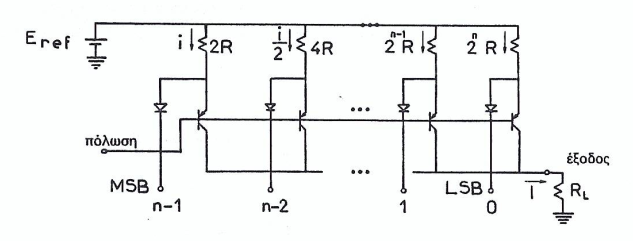
\includegraphics[width=\linewidth]{DArevma.png}
    \caption{Απλός μετατροπέας $D/A$ ρεύματος. Έχει πολλά μειονεκτήματα, όπως σημαντική εξάρτηση από θερμοκρασία, μεγάλη διαφορά στις τιμές των αντιστάσεων κλπ.}
    \label{DArevmatos}
\end{figure}

\emph{Σελ. 470-1}

\subsection{Να περιγραφεί η αρχή λειτουργίας ενός μετατροπέα $D/A$ \newlineτάσης.}
Οι μετατροπείς $D/A$ μετατρέπουν ένα ψηφιακό σήμα σε αναλογικό συγκρίνοντας την αναλογική τάση που αντιπροσωπεύει το ψηφιακό σήμα με την τάση αναφοράς. Για ψηφιακή λέξη $8bit$ έχουμε
έξοδο: 

\begin{align*}
    \upsilon = K E_{ref} \left( b_7/2 + b_6/4 + b_5/8 + b_4/16 +b_3/32 + b_2/64 + b_1/128 + b_0/256 \right)
\end{align*}

Έστω ότι η είσοδος είναι 00000001. Ένα δυαδικό 1 συνδέει τον αντίστοιχο διακόπτη στη θέση 1 (δηλαδή στο αρνητικό άκρο της πηγής αναφοράς, Σχήμα \ref{DAtashs}). Έτσι
μόνο η 1η αντίσταση συνδέεται στην πηγή αναφοράς ενώ οι άλλες αντιστάσεις συνδέονται στη γη. Κατά συνέπεια η έξοδος θα είναι $\upsilon = -\frac{E_{ref}}{256R}R_o$. Αν η είσοδος είναι
00000011, $\upsilon = -3\frac{E_{ref}}{256R}R$.

\begin{figure}
    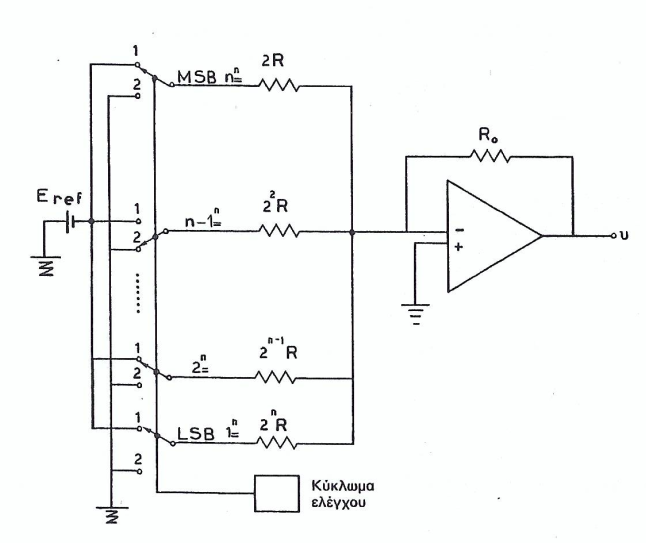
\includegraphics[width=\linewidth]{DAtashs.png}
    \caption{Μια απλή διάταξη μετατροπέα $D/A$ τάσης}
    \label{DAtashs}
\end{figure}

\emph{Σελ. 469-70}

\subsection{Τι είναι χρόνος αποκατάστασης σε έναν μετατροπέα $D/A$?}
Ο χρόνος που μεσολαβεί εώς ότου η έξοδος φτάσει την τελική τιμή με ακρίβεια $\pm1/2LSB$. Aυτόν τον χρόνο εννοούμε όταν λέμε χρόνος μετατροπής. Εξαρτάται από το είδος
των διακοπτών, το είδος των αντιστατών (αν έχουν αυτεπαγωγή ή όχι) και από τον ενισχυτή εξόδου (αν υπάρχει). Προδιαγράφεται για μια ορισμένη χωρητικότητα στην έξοδο.

\emph{Σελ. 473}

\end{document}
